\section{Training Protocols}

In the realm of sport horse training, the development and implementation of effective training protocols are paramount to ensure optimal fitness and welfare. Training protocols encompass a structured framework that guides the progressive conditioning and skill enhancement of sport horses. These protocols are tailored to address specific objectives, taking into account factors such as discipline, competition level, and individual horse characteristics. 

The design of training protocols requires a comprehensive understanding of equine physiology, biomechanics, and the principles of exercise science. Additionally, it necessitates an appreciation for the horse's physical and mental capabilities, as well as the ability to adapt protocols to accommodate individual variations. The systematic and methodical nature of training protocols ensures a gradual progression, allowing horses to adapt to increasing demands while minimizing the risk of injury and fatigue. Consequently, the implementation of well-designed training protocols serves as an important factor in optimizing the athletic potential and overall well-being of sport horses.

This thesis concentrates on several common disciplines in which horses compete. These disciplines are eventing, dressage, showjumping, and endurance. Eventing is a triathlon-like equestrian competition comprising three phases: dressage, cross-country, and showjumping. In dressage, horses execute a series of predetermined movements within a defined arena. Movements include precise turns, circles, lateral movements, and special gaits. The cross-country phase involves negotiating a course with natural obstacles over varied terrain. Showjumping is a timed competition where horses navigate a course of fixed obstacles. The objective is to complete the course with the fewest penalties, with penalties incurred for knockdowns, refusals, or exceeding the time limit. The technical aspects of jumping, such as take-off and landing, determine the overall performance assessment. Furthermore, endurance riding is a test of stamina and endurance, covering long distances often in natural and challenging terrains. These remarkable horses are known for their ability to maintain a steady pace over extended periods.

Among the diverse array of training protocols, \gls{set} is of particular importance. \gls{set} is a structured training program that aims to evaluate fitness and identify fatigue by inducing biomechanical and physiologic changes. They are designed to align with the discipline and are routinely used for physiological response assessment. The assessment encompasses the measurement of key physiological variables, offering insights into the horse's physical exertion and metabolic demands. Then, the insights are used for performance monitoring, exercise planning, and fitness determination. Designing and planning exercises in accordance with the \gls{set} results may decrease the risk of overloading and overtraining injuries \cite{graaf232}.

\gls{set}s can be performed on treadmills or in the field \cite{munsters_2014_exercise}. Performing \gls{set} on treadmills offers a few advantages that are mentioned in chapter \ref{datacollection-devices}. Treadmill-based assessments provide a controlled environment where precise measurements can be obtained. This controlled setting allows for consistent speed and incline, reducing confounding variables. On the other hand, performing \gls{set} on the field resembles real-world competition and racing situations in a natural environment. It offers a more holistic assessment of the horse's fitness and performance. Field-based \gls{set}s expose horses to varying terrains, outdoor elements, and contextual factors that are integral to their training and competitive environments. Therefore, \gls{set}s performed on the field enables a more accurate evaluation of the horse's adaptability, endurance, and ability to perform under realistic conditions.

Blood \gls{lac} is one of the important physiological variables measured during a SET. Even though the measurement of blood \gls{lac} consists of an invasive procedure involving the extraction of a blood sample from the jugular vein (as mentioned in chapter \ref{datacollection-devices}), it serves as a crucial indicator of muscle adaptation to the imposed training workload and provides valuable insights into the subject's fatigue level over time.

For the purpose of data collection in this study, \gls{set} was chosen as the designated training protocol. This selection aligns with our primary objective of evaluating fitness levels, with a specific focus on incorporating the measurement of a crucial fatigue-related parameter, blood \gls{lac}. 

To ensure the reliability, portability, and versatility required for fitness monitoring, the collection of data during SET involved the utilization of body-mounted \gls{imu}s and \gls{hr} monitoring devices. These devices were selected following an eligibility assessment for reliability, portability, and versatility. In the forthcoming sections, a comprehensive account of the data collection protocol will be presented, encompassing details regarding the participating subjects and the structural framework employed for organizing the collected data.

\subsection{SETs} \label{sec:trainingprotocol}

In general, \gls{set}s are designed in accordance with the discipline in which the horse is competing. Therefore, in this study, a \gls{set} was assigned for each discipline, which is described in the following. Throughout the \gls{set}, horses demonstrated a range of diverse and distinct gaits. For the precise definitions of each gait, please refer to Table \ref{tab:gait} and Figure \ref{fig:horseshoe}. It should be noted that right before performing the \gls{set} for all horses, resting plasma \gls{lac} was measured.

\begin{table}[!htb] 
\centering
\caption{Description of gaits used in this book. The type of gait indicates if the horse can perform the gait without (natural) or with (artificial) learning. The footfall patterns are illustrated in Figure \ref{fig:horseshoe}}% Add 'table' caption
\resizebox{\linewidth}{!}{%
\begin{tabular}{p{1cm}p{1.5cm}p{10cm}}
\toprule
\textbf{Gait} & \textbf{Type} & \textbf{Definition} \\
\midrule 

Walk  & Natural  & A lateral symmetrical gait consists of four-beat rhythm with the hoof land and take off in the following sequence: left hind hoof, left front hoof, right hind hoof, right front hoof.\\

Trot  & Natural  & A diagonal symmetrical gait consists of two-beat diagonal rhythm. The right front hoof and left hind hoof rise and fall together alternately with the diagonal pair left front hoof and right hind hoof. \\

Pace  & Natural  & A lateral gait characterized by a two-beat lateral pattern. In a pace gait, the horse moves its hooves on one side of its body together, followed by the hooves on the opposite side. It is a gait commonly associated with certain horse breeds, such as Standardbred trotters and Icelandic horses, and is known for its smoothness and speed. \\

Canter  & Natural  & An asymmetric gait, consists of three-beat rhythm with the following sequence: left hind hoof, right hind hoof and left front hoof simultaneously, right front hoof for right lead canter. For left lead canter,  right hind hoof, right front hoof and left hind hoof simultaneously, left front hoof. \\

Tölt  & Natural  & A four-beat gait, hooves strike the ground in a specific sequence: right hind, right front, left hind, left front. It is a distinctive gait predominantly associated with Icelandic horses, known for its smooth and comfortable motion. It lacks a suspension phase, distinguishing it from the trot, and can be performed at various speeds. \\

Passage  & Artificial  & A measured, very collected, elevated and cadenced trot \cite{clayton_2019_a}. One of the important gait types that can be learned by dressage horses. \\

Piaffe  & Artificial  & A highly collected, cadenced, elevated diagonal movement in place or nearly in place \cite{clayton_2019_a}, specifically for dressage horses.\\
\bottomrule 
\label{tab:gait}
\end{tabular}}
\end{table}

\begin{figure}[!tbp]
\centering
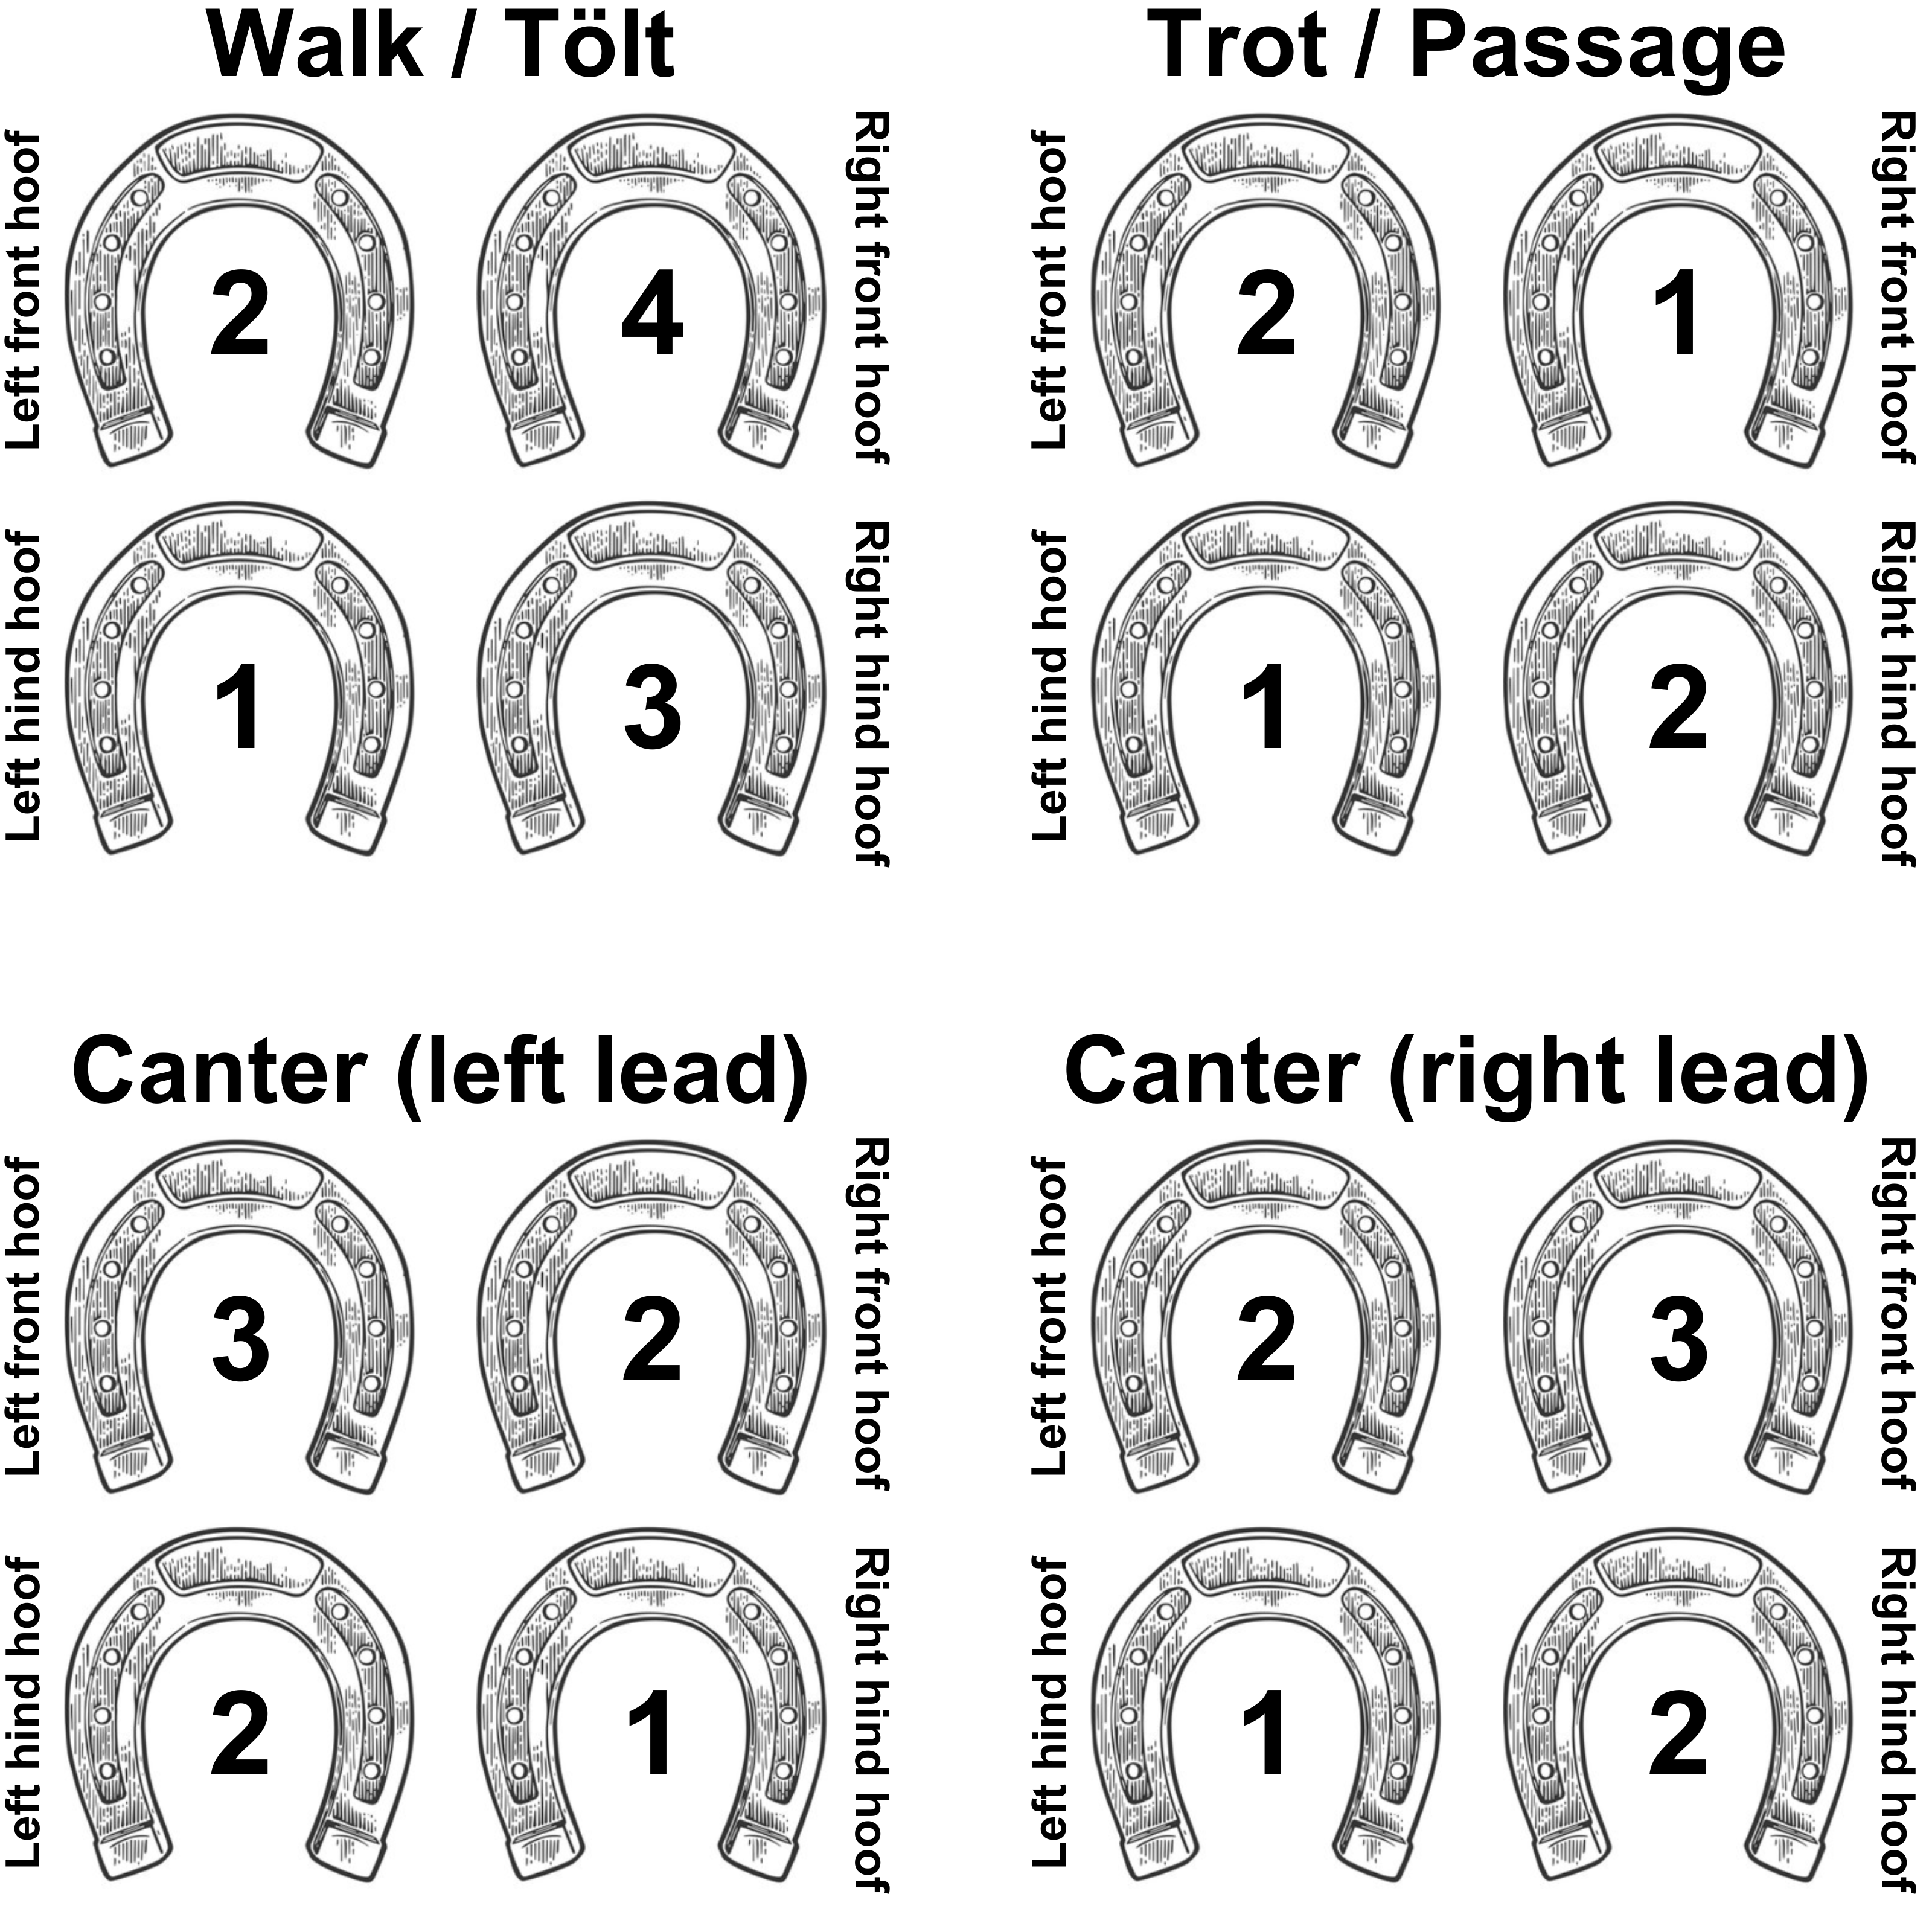
\includegraphics[scale=0.1]{chapters/data/figures/Horseshoe.png}
\caption{Illustration of footfall patterns for gaits that were described in Table \ref{tab:gait}.}
\label{fig:horseshoe}
\end{figure}

\vspace{10pt}
{\noindent\textbf{Eventing SET} \par}
Eventing horses performed their designated \gls{set} on a 1000 m outdoor racetrack with sand footing. The order of \gls{set} tasks is depicted in Figure \ref{fig:eventingset}. To present the collected data from an \gls{imu} over the duration of a \gls{set}, Figure \ref{fig:IMUsignals} in Appendix \ref{appendix:appendix2}, illustrates the acceleration signals recorded from the sacrum \gls{imu} of an eventing horse throughout the \gls{set}. The \gls{set} started with a warm-up walk (10 minutes) and trot (5 minutes), followed by four incremental exercise steps and finished by a cool-down walk (10 minutes) \cite{CBM}. Incremental steps consisted of 1000 m canter at speeds 5.8, 6.7, 7.5, and 9.2 m/s (or at a horse’s maximal speed), which were controlled by riders using \gls{gps} \cite{munsters_2014_exercise}. After each step, horses were slowed down and walked for five minutes, and within the walking, horses were briefly stopped (5 to 15 seconds) and blood samples were collected. If the plasma \gls{lac} exceeded 4 \gls{mmol/L}, the subsequent incremental steps were omitted, and the \gls{set} was terminated with the cool-down \cite{MUNSTERS2013193}. Finally, a blood sample was also taken right after a cool-down walk to measure the recovery plasma \gls{lac}.

\begin{figure}[!htbp]
\centering
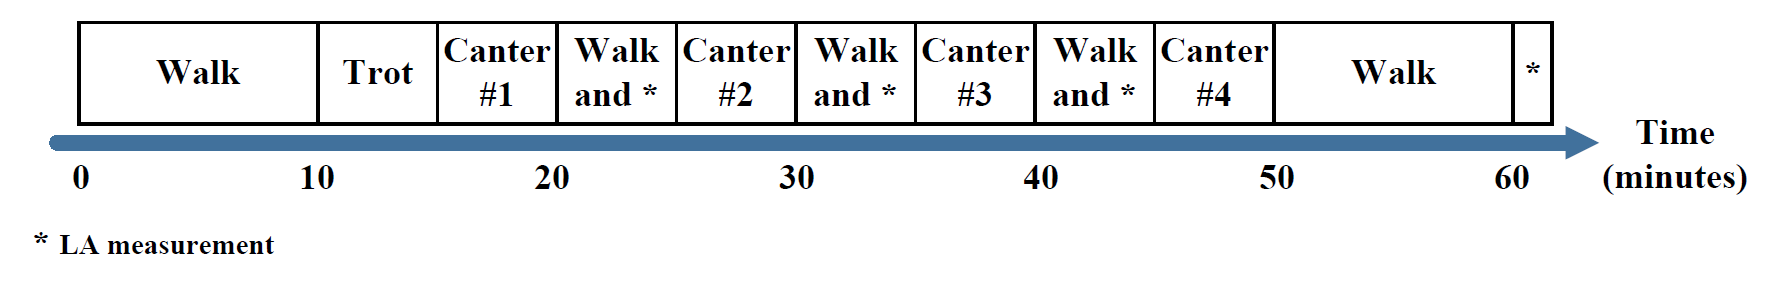
\includegraphics[scale=0.27]{chapters/data/figures/EventingSET.png}
\caption{Order of the tasks for eventing and showjumping horses to perform the designated \gls{set}. In addition to these tasks, showjumping horses also performed a few more tasks, illustrated in Figure \ref{fig:showjumpingset}}
\label{fig:eventingset}
\end{figure}

\vspace{5pt}
{\noindent\textbf{Showjumping SET} \par}
Similar to eventing \gls{set}, showjumping horses performed a \gls{set} consisted of an order warm-up walk (5 minutes) and trot (10 minutes), four 1000 m cantering incremental steps (5.8, 6.7, 7.5, and 9.2 m/s), and recovery walk (5 minutes). After each incremental step and recovery walk, a blood sample was collected for plasma \gls{lac}measurement. After the recovery walk, as shown in Figure \ref{fig:showjumpingset}, the \gls{set} continued with a few jumping-related steps, which were: rider-free trot/canter (2 minutes) including jumping over five random fences, five jumps over fences with 60 cm height (7.1 m/s), walk (2 minutes) and plasma \gls{lac} measurement in between, five jumps over fences with 80 cm height (7.1 m/s), plasma \gls{lac} measurement, recovery walk (10 minutes), and the last plasma \gls{lac} measurement. Depending on the rider or horse's experience, the height of 60 and 80 cm fences might be reduced to 40 and 60 cm respectively. The arena dimension was 20 m * 60 m and on each long side, five fences with a width of 3.35 m were located (10 fences in total).



\begin{figure}[!htbp]
\centering
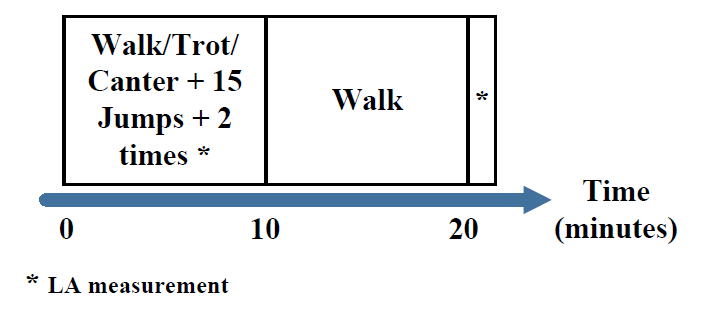
\includegraphics[scale=0.3]{chapters/data/figures/ShowjumpingSET.png}
\caption{Order of the additional tasks for showjumping horses to perform the designated \gls{set}. The main part of their SET was depicted in Figure \ref{fig:eventingset}}
\label{fig:showjumpingset}
\end{figure}

\vspace{5pt}
{\noindent\textbf{Dressage SET} \par}
Dressage horses performed two \gls{set}s on indoor arenas with sand surfaces. The first \gls{set} consisted of skills that are presented during competitions, including special types of walk, trot, canter, passage, and piaffe. The tasks for second \gls{set} are illustrated in Figure \ref{fig:dressageset}, which were performed as follows: left-lead walk (2 minutes), right-lead walk (2 minutes), right-lead trot (2 minutes), left-lead trot (2 minutes), blood sample collection for plasma \gls{lac} measurement, left-lead canter (2 minutes, 5.0 m/s), right-lead canter (2 minutes, 5.0 m/s), blood sample collection for plasma \gls{lac} measurement, recovery walk (3 minutes), rider's choice trot and canter (15 minutes), blood sample collection for plasma \gls{lac} measurement \cite{MUNSTERS2013193}. 

\begin{figure}[!htbp]
\centering
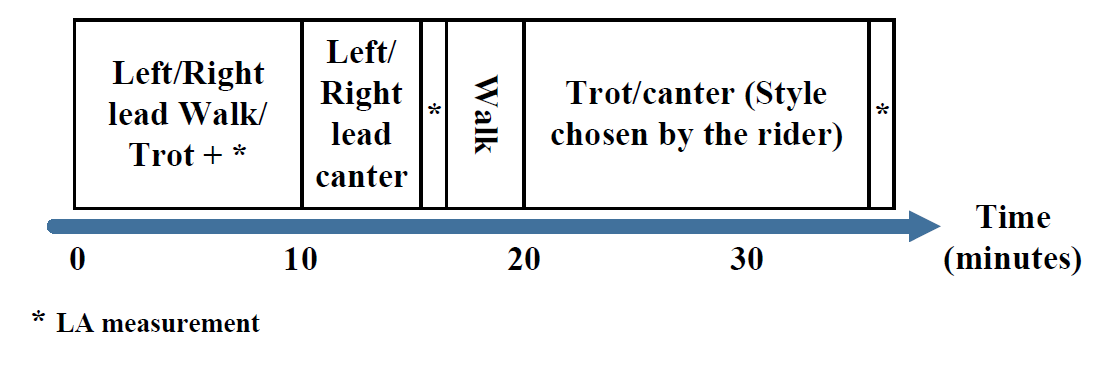
\includegraphics[scale=0.30]{chapters/data/figures/DressageSET.png}
\caption{The tasks of Second Dressage SET}
\label{fig:dressageset}
\end{figure}

\vspace{5pt}
{\noindent\textbf{Endurance SET} \par}
Similar to the eventing and dressage horses, the endurance horses also performed the \gls{set} on a sand race track. The \gls{set} tasks are illustrated in Figure \ref{fig:enduranceset}, which started with a warm-up walk (10 minutes) and a trot (10 minutes). Then, it was followed by one incremental step of cantering over 27 km at 6 m/s, and two incremental steps of cantering over 1500 m at 7.5 and 8.8 m/s. Between every three incremental steps, 700 m of a slow-trot was performed as recovery. Finally, the \gls{set} was finished with a 10-minute recovery walk. The blood samples for plasma \gls{lac} measurements were drawn after each incremental step within 30 seconds and once after the final recovery walk \cite{fraipont}.

\begin{figure}[!htbp]
\centering
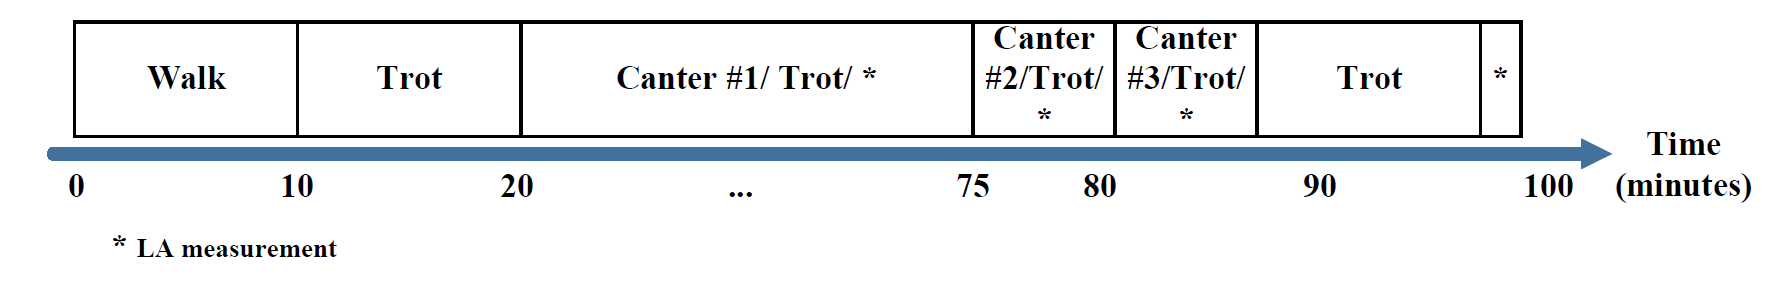
\includegraphics[scale=0.27]{chapters/data/figures/EnduranceSET.png}
\caption{Order of the tasks for endurance horses to perform the designated \gls{set}.}
\label{fig:enduranceset}
\end{figure}